\chapter{Data}
\label{ch:appendix-data}

Complementing the discussion of the introduced datasets in Chapter
\ref{ch:data}, we additionally discuss the 2D rectangle dataset originally
used to prototype the proposed shape completion approaches.
Additionally, we provide further examples for the remaining datasets.

\section{2D Example}
\label{sec:appendix-data-2d}

% TODO process flow figure:
% - create and rotate rectangles, compute representations
% - setup a camera "seeing" the rectangles
% - perform ray tracing
% - perform noisy ray tracing.
% TODO make x, y explicit!
\begin{figure}
  \centering
  \vspace*{-0.75cm}
  \begin{subfigure}[t]{1\textwidth}
    \centering
    \begin{tikzpicture}
      \node[] at (0, 2.5) {\small\begin{tabular}{c}sample\\rectangle\end{tabular}};
      \node[] at (0,0) {\includegraphics[height=2.5cm]{data/2d/validation_0_proc1}};
      \node at (0, -1.5) {\small Shape $y^*$};

      \node[] at (4,2.5) {\small\begin{tabular}{c}camera pose\\$t_{\text{cam}}; r_{\text{cam}}$\end{tabular}};
      \node[] at (4,-1) {\includegraphics[width=3.75cm]{data/2d/validation_0_proc2}};
      
      %\node[] at (9.5,2.5) {\begin{tabular}{c}noise\\$\theta_{\text{hit}} = 1; \theta_{\text{ignore}} = 0$\end{tabular}};
      \node at (9.75, 2.75) {\small Observation $x$};
      \draw[-,dashed] (7.2,2.25) rectangle (12.3, -4.75);

      \node at (8.5, 1.65) {\footnotesize\begin{tabular}{c}Observed\\Points\end{tabular}};
      \node at (11, 1.65) {\footnotesize\begin{tabular}{c}Full\\Free Space\end{tabular}};
      \node[] at (8.5,0) {\includegraphics[height=2.5cm]{data/2d/validation_0_proc3}};
      \node[] at (11,0) {\includegraphics[height=2.5cm]{data/2d/validation_0_proc4}};
      \node[] at (11,-2.5) {\includegraphics[height=2.5cm]{data/2d/validation_0_proc5}};
      \node at (11, -4.15) {\footnotesize\begin{tabular}{c}Partial\\Free Space\end{tabular}};

      \draw[->] (0,2) -- (0,1.3);
      \draw[->] (1.25,0) -- (2.25,0);
      \draw[->] (4,2) -- (4,1.3);
      \draw[->] (5.75, 0) -- (7.15,0);
      %\draw[->] (9.5,2) -- (9.5,1.3);
      
      \node at (1.75,0.3) {\small(a)};
      \node at (6.5,0.3) {\small(b)};
      
      \node at (2.5,-4.7) {\small(c)\hspace{0.75cm} Corresponding (Signed) Distance Functions};
      \draw[-,dashed] (-2,-5) -- (13,-5);
      
      \node[] at (0,-6.5) {\includegraphics[height=2.5cm]{data/2d/validation_0_proc6}};
      %\node at (0, -8) {\small $\text{sdf}(y^*)$};

      \node[] at (8.5,-6.5) {\includegraphics[height=2.5cm]{data/2d/validation_0_proc7}};
      \node[] at (11,-6.5) {\includegraphics[height=2.5cm]{data/2d/validation_0_proc8}};
      \node[] at (8.5,-9) {\includegraphics[height=2.5cm]{data/2d/validation_0_proc9}};
    \end{tikzpicture}
    % TODO short caption
    \subcaption{Illustration of the data generation process for our 2D rectangle
    dataset. We sample random rectangles $y \in \mathbb{R}^{H \times W}$ with
    different size and rotation. Then, indicated with (a), we set up a
    1D camera given the corresponding center $t_{\text{cam}}$ and viewing direction
    $r_{\text{cam}}$, \cf Figure \ref{fig:appendix-data-2d-camera}. Subsequently,
    marked by (b), we perform ray tracing to compute the observation
    $x \in \mathbb{R}^{H \times W}$ in the form of observed points, full free space
    and partial free space. In (c), we post-process the shapes $y^*$ as well as the
    observations $x$ to obtain the corresponding (signed) distance functions.}
    \label{fig:appendix-data-2d}
  \end{subfigure}\\[0.5cm]
  \begin{subfigure}[t]{1\textwidth}
    \centering
    % https://tex.stackexchange.com/questions/123760/draw-crosses-in-tikz
    \tikzset{cross/.style={cross out, draw=black, minimum size=2*(#1-\pgflinewidth), inner sep=0pt, outer sep=0pt},cross/.default={0.1cm}}
    \begin{tikzpicture}
      \node[cross] (c) at (0,0) {};
      \node at (-0.25,-0.25) {$t_{\text{cam}}$};
      
      \draw[-] (1,-1.5) -- (1,1.5);
      %\draw[-] (0,0) -- (0.5,0.5);
      \draw[-,dashed,draw=black!40] (0,0) -- (1.5,1.5);
      %\draw[-] (0,0) -- (0.5,-0.5);
      \draw[-,dashed,draw=black!40] (0,0) -- (1.5,-1.5);
      %\draw[-] (0.5,0.5) -- (0.5,-0.5);
      
      \draw[->] (0,0) -- (3,0);
      \node[] at (2,0.25) {$r_{\text{cam}}$};
      
      \draw [decorate,decoration={brace,amplitude=5pt}]
  (0.05,0.15) -- (0.95,0.15);
      \node at (0.5, 0.6) {$f$};

      \draw[->] (-1,-2) -- (-1,-1) node at (-1,-0.75) {$y$};
      \draw[->] (-1,-2) -- (0,-2) node at (0.25,-2) {$x$};
      
      \node[minimum width=2cm,minimum height=1.5cm,rotate=30,draw=black,rectangle] (r) at (5,-0.5){};
      
      \draw[->] (c) -- (r);
      \node at (3.65,0) {$p$};
    \end{tikzpicture}
    % TODO short caption
    \subcaption{Illustration of the 1D camera from Definition \ref{def:appendix-data-2d-camera}.
    The camera is set up by specifying the camera center $t_{\text{cam}}$ and
    the corresponding viewing direction $r_{\text{cam}}$ which is used to
    derive the rotation matrix $\mathcal{R}_{\text{cam}}$.}
    \label{fig:appendix-data-2d-camera}
  \end{subfigure}
  \vskip 12px

  \caption{Illustration of the data generation process in Figure \ref{fig:appendix-data-2d} and
  the used camera model in Figure \ref{fig:appendix-data-2d-camera}.}
\end{figure}

Our synthetic 2D dataset consists of arbitrarily scaled and rotated rectangles.
Because we work with either occupancy grids or signed distance functions,
the rectangles are directly generated in discretized forms, \ie as binary images.
This way we can directly generate the shape set $\mathcal{Y}\subseteq \mathbb{R}^{H \times W}$
used to learn the shape prior as well as the ground truth shapes $\mathcal{Y}^* \subseteq \mathbb{R}^{H \times W}$.
We note that $\mathcal{Y} \cap \mathcal{Y}^* = \emptyset$, \ie we assume that the
shape prior is not trained on the same shapes also encountered during shape completion.
It remains to synthesize the observations $\mathcal{X}\subseteq \mathbb{R}^{H \times W}$
from the ground truth shapes $\mathcal{Y}$*. These are obtained through
a ray tracing process given a 1D projective camera. The overall process
is also illustrated in Figure \ref{fig:appendix-data-2d} and the ray tracing
part is described in detail in the following.

\subsection{Ray Tracing}

Given the discretized shapes $\mathcal{Y}^* \subseteq \mathbb{R}^{H \times W}$, we
place a 1D projective camera in the scene in order to record a
1D projection of the shapes which can subsequently be back-projected to
form the observations $\mathcal{X}$:

% TODO cite
% TODO projective matrix P?
\begin{definition}
  \label{def:appendix-data-2d-camera}
  A 1D projective camera is described by a tuple $(\mathcal{K}, \mathcal{R}, t)$
  where $\mathcal{K} \in \mathbb{R}^{2\times 2}$ is the intrinsic camera matrix and
  $\mathcal{R} \in \mathbb{R}^{2 \times 2}$, $t \in \mathbb{R}^2$ define
  a similarity in 2D. The intrinsic camera matrix has the form
  \begin{align}
    \mathcal{K} = \left[\begin{matrix}f & u\\ 0 & 1\end{matrix}\right]
  \end{align}
  and $\mathcal{R}$ is orthogonal.
  % TODO wording principal point ...
  Here, $f$ is the focal length, \ie
  the distance between camera center and virtual image line; $u$ is the
  principal point, \ie center pixel, in 1D image coordinates --  we always
  assume $u$ to be the middle pixel of the 1D image, thereby also defining the
  resolution as $2u$.
\end{definition}

The above definition is illustrated in Figure \ref{fig:appendix-data-2d-camera}.
Given a camera $(\mathcal{K}, \mathcal{R}, t)$, the overall projection matrix is
\begin{align}
  \mathcal{P} = \mathcal{K}\left[\begin{matrix} \mathcal{R} & t\end{matrix}\right] \in \mathbb{R}^{2 \times 3}.
\end{align}
However, for ray tracing, we are interested in the inverse transformation \cite[Chapter~6]{HartleyZisserman:2006}
\begin{align}
  \mathcal{P}^+ = (\mathcal{P}^T \mathcal{P})^{-1} \mathcal{P}^T \in \mathbb{R}^{3 \times 2}
  \label{eq:data-2d-pinv}
\end{align}
which gives the ray going through the camera center
and pixel $x = (x_1, 1)^T$:
\begin{align}
  r = \left[\begin{matrix}
    \frac{\tilde{r}_1}{\tilde{r}_3}\\
    \frac{\tilde{r}_2}{\tilde{r}_3}\\
    1
  \end{matrix}\right]
  \quad\text{ with }\quad \tilde{r} = \mathcal{P}^+ x.
\end{align}
To set up $\mathcal{P}^+$, we randomly choose a camera position $t_{\text{cam}}$
within appropriate ranges and compute the corresponding viewing direction $r_{\text{cam}}$
letting the camera look to the center of our shapes. Then,
following \cite[Chapter~6]{HartleyZisserman:2006}:
\begin{align}
  \mathcal{R} = \mathcal{R}_{\text{cam}}^T\quad\text{ and }\quad t = \mathcal{R}t_{\text{cam}}.
\end{align}
where the matrix $\mathcal{R}_{\text{cam}}$ corresponding to the camera's viewing
direction $r_{\text{cam}}$ can be set up given the angle
$\alpha = \angle(r_{\text{cam}}, (1,0)^T)$ between viewing direction and
x-axis:
\begin{align}
  \mathcal{R}_{\text{cam}} = \left[\begin{matrix}
    \cos \alpha & -\sin \alpha\\
    \sin \alpha & \cos \alpha
  \end{matrix}\right]
\end{align}.
Using $\mathcal{R}$, $t$ as well as the intrinsic camera matrix $\mathcal{K}$,
which we fix in advance, $\mathcal{P}^+$ is computed following Equation \eqref{eq:data-2d-pinv}.

Ray tracing is then performed by taking each pixel in homogeneous coordinates,
computing the corresponding ray and following it to determine all intersected
pixels of the binary image until it hits an occupied pixel. All pixels up to the
occupied pixel are marked as free space. If we also consider rays that leave
the image without hitting an occupied pixel, we obtain the full free space;
if we only consider rays to occupied pixels, we obtain the partial free space,
see Figure \ref{fig:appendix-data-2d-examples-1} for examples regarding this distinction.
The distinction becomes important on real data, \eg on KITTI
\cite{GeigerLenzUrtasun:2012,GeigerLenzStillerUrtasun:2013},
where full free space cannot be computed reliably.

\subsection{Noise}

% TODO different color, not red!
\begin{figure}
  \centering
  \begin{subfigure}[]{0.125\textwidth}
    \vfill
    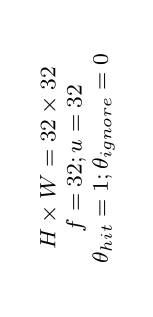
\begin{tikzpicture}
      \node[rotate=90] at (0,0) {
        \footnotesize
        \begin{tabular}{c}
          $H \times W = 32 \times 32$\\
          $f = 32; u = 32$\\
          $\theta_{\text{hit}} = 1; \theta_{\text{ignore}} = 0$
        \end{tabular}
      };
    \end{tikzpicture}
    \vfill
  \end{subfigure}
  \begin{subfigure}[t]{0.25\textwidth}
    \begin{subfigure}[t]{0.49\textwidth}
      \includegraphics[width=2cm]{data/2d/default/validation_0_output}
    \end{subfigure}\hfill
    \begin{subfigure}[t]{0.49\textwidth}
      \includegraphics[width=2cm]{data/2d/default/validation_0_input}
    \end{subfigure}\\[-2px]
    \begin{subfigure}[t]{0.49\textwidth}
      \includegraphics[width=2cm]{data/2d/default/validation_0_space}
    \end{subfigure}\hfill
    \begin{subfigure}[t]{0.49\textwidth}
      \includegraphics[width=2cm]{data/2d/default/validation_0_real_space}
    \end{subfigure}
  \end{subfigure}
  \begin{subfigure}[t]{0.25\textwidth}
    \begin{subfigure}[t]{0.49\textwidth}
      \includegraphics[width=2cm]{data/2d/default/validation_1_output}
    \end{subfigure}\hfill
    \begin{subfigure}[t]{0.49\textwidth}
      \includegraphics[width=2cm]{data/2d/default/validation_1_input}
    \end{subfigure}\\[-2px]
    \begin{subfigure}[t]{0.49\textwidth}
      \includegraphics[width=2cm]{data/2d/default/validation_1_space}
    \end{subfigure}\hfill
    \begin{subfigure}[t]{0.49\textwidth}
      \includegraphics[width=2cm]{data/2d/default/validation_1_real_space}
    \end{subfigure}
  \end{subfigure}
  \begin{subfigure}[t]{0.25\textwidth}
    \begin{subfigure}[t]{0.49\textwidth}
      \includegraphics[width=2cm]{data/2d/default/validation_3_output}
    \end{subfigure}\hfill
    \begin{subfigure}[t]{0.49\textwidth}
      \includegraphics[width=2cm]{data/2d/default/validation_3_input}
    \end{subfigure}\\[-2px]
    \begin{subfigure}[t]{0.49\textwidth}
      \includegraphics[width=2cm]{data/2d/default/validation_3_space}
    \end{subfigure}\hfill
    \begin{subfigure}[t]{0.49\textwidth}
      \includegraphics[width=2cm]{data/2d/default/validation_3_real_space}
    \end{subfigure}
  \end{subfigure}\\
  \begin{subfigure}[]{0.125\textwidth}
    \vfill
    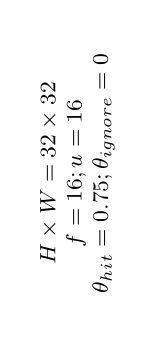
\begin{tikzpicture}
      \node[rotate=90] at (0,0) {
        \footnotesize
        \begin{tabular}{c}
          $H \times W = 32 \times 32$\\
          ${f = 16; u = 16}$\\
          $\theta_{\text{hit}} = 0.75; \theta_{\text{ignore}} = 0$
        \end{tabular}
      };
    \end{tikzpicture}
    \vfill
  \end{subfigure}
  \begin{subfigure}[t]{0.25\textwidth}
    \begin{subfigure}[t]{0.49\textwidth}
      \includegraphics[width=2cm]{data/2d/32_resolution/validation_0_output}
    \end{subfigure}\hfill
    \begin{subfigure}[t]{0.49\textwidth}
      \includegraphics[width=2cm]{data/2d/32_resolution/validation_0_input}
    \end{subfigure}\\[-2px]
    \begin{subfigure}[t]{0.49\textwidth}
      \includegraphics[width=2cm]{data/2d/32_resolution/validation_0_space}
    \end{subfigure}\hfill
    \begin{subfigure}[t]{0.49\textwidth}
      \includegraphics[width=2cm]{data/2d/32_resolution/validation_0_real_space}
    \end{subfigure}
  \end{subfigure}
  \begin{subfigure}[t]{0.25\textwidth}
    \begin{subfigure}[t]{0.49\textwidth}
      \includegraphics[width=2cm]{data/2d/32_resolution/validation_1_output}
    \end{subfigure}\hfill
    \begin{subfigure}[t]{0.49\textwidth}
      \includegraphics[width=2cm]{data/2d/32_resolution/validation_1_input}
    \end{subfigure}\\[-2px]
    \begin{subfigure}[t]{0.49\textwidth}
      \includegraphics[width=2cm]{data/2d/32_resolution/validation_1_space}
    \end{subfigure}\hfill
    \begin{subfigure}[t]{0.49\textwidth}
      \includegraphics[width=2cm]{data/2d/32_resolution/validation_1_real_space}
    \end{subfigure}
  \end{subfigure}
  \begin{subfigure}[t]{0.25\textwidth}
    \begin{subfigure}[t]{0.49\textwidth}
      \includegraphics[width=2cm]{data/2d/32_resolution/validation_3_output}
    \end{subfigure}\hfill
    \begin{subfigure}[t]{0.49\textwidth}
      \includegraphics[width=2cm]{data/2d/32_resolution/validation_3_input}
    \end{subfigure}\\[-2px]
    \begin{subfigure}[t]{0.49\textwidth}
      \includegraphics[width=2cm]{data/2d/32_resolution/validation_3_space}
    \end{subfigure}\hfill
    \begin{subfigure}[t]{0.49\textwidth}
      \includegraphics[width=2cm]{data/2d/32_resolution/validation_3_real_space}
    \end{subfigure}
  \end{subfigure}
  \begin{subfigure}[]{0.125\textwidth}
    \vfill
    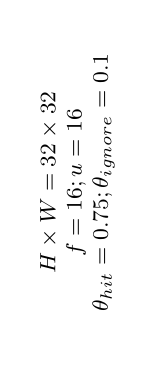
\begin{tikzpicture}
      \node[rotate=90] at (0,0) {
        \footnotesize
        \begin{tabular}{c}
          $H \times W = 32 \times 32$\\
          ${f = 16; u = 16}$\\
          ${\theta_{\text{hit}} = 0.75; \theta_{\text{ignore}} = 0.1}$
        \end{tabular}
      };
    \end{tikzpicture}
    \vfill
  \end{subfigure}
  \begin{subfigure}[t]{0.25\textwidth}
    \begin{subfigure}[t]{0.49\textwidth}
      \includegraphics[width=2cm]{data/2d/32_resolution_noise/validation_0_output}
    \end{subfigure}\hfill
    \begin{subfigure}[t]{0.49\textwidth}
      \includegraphics[width=2cm]{data/2d/32_resolution_noise/validation_0_input}
    \end{subfigure}\\[-2px]
    \begin{subfigure}[t]{0.49\textwidth}
      \includegraphics[width=2cm]{data/2d/32_resolution_noise/validation_0_space}
    \end{subfigure}\hfill
    \begin{subfigure}[t]{0.49\textwidth}
      \includegraphics[width=2cm]{data/2d/32_resolution_noise/validation_0_real_space}
    \end{subfigure}
  \end{subfigure}
  \begin{subfigure}[t]{0.25\textwidth}
    \begin{subfigure}[t]{0.49\textwidth}
      \includegraphics[width=2cm]{data/2d/32_resolution_noise/validation_1_output}
    \end{subfigure}\hfill
    \begin{subfigure}[t]{0.49\textwidth}
      \includegraphics[width=2cm]{data/2d/32_resolution_noise/validation_1_input}
    \end{subfigure}\\[-2px]
    \begin{subfigure}[t]{0.49\textwidth}
      \includegraphics[width=2cm]{data/2d/32_resolution_noise/validation_1_space}
    \end{subfigure}\hfill
    \begin{subfigure}[t]{0.49\textwidth}
      \includegraphics[width=2cm]{data/2d/32_resolution_noise/validation_1_real_space}
    \end{subfigure}
  \end{subfigure}
  \begin{subfigure}[t]{0.25\textwidth}
    \begin{subfigure}[t]{0.49\textwidth}
      \includegraphics[width=2cm]{data/2d/32_resolution_noise/validation_3_output}
    \end{subfigure}\hfill
    \begin{subfigure}[t]{0.49\textwidth}
      \includegraphics[width=2cm]{data/2d/32_resolution_noise/validation_3_input}
    \end{subfigure}\\[-2px]
    \begin{subfigure}[t]{0.49\textwidth}
      \includegraphics[width=2cm]{data/2d/32_resolution_noise/validation_3_space}
    \end{subfigure}\hfill
    \begin{subfigure}[t]{0.49\textwidth}
      \includegraphics[width=2cm]{data/2d/32_resolution_noise/validation_3_real_space}
    \end{subfigure}
  \end{subfigure}
  % TODO short caption
  \caption{Examples from our synthetic 2D dataset with different resolutions of
  the 1D image, \ie $64$ and $32$, and difference noise parameters, \ie
  $\theta_{\text{hit}} \in \{1, 0.7\}$ and $\theta_{\text{ignore}} \in \{0, 0.2\}$.
  For each example, we show the full shape $y$ and the observation $x$
  in the form of observed points, free space from all rays (\ie full free space)
  and free space from rays corresponding to observed points (\ie partial free space).}
  \label{fig:appendix-data-2d-examples-1}
\end{figure}

So far, the ray tracing approach is fully deterministic. Although we can
reduce the resolution of the 1D image thereby reducing the number of observed
pixels, we also want to inject some randomness into ray tracing to
simulate real conditions. To this end, we introduce two probabilities
$\theta_{\text{hit}}$ and $\theta_{\text{ignore}}$ describing the probability
that a ray actually hits an occupied pixel and the probability that
all occupied pixels along a ray are ignored, respectively. Examples are provided
in Figure \ref{fig:appendix-data-2d-examples-1}.

\subsection{Discussion}

% TODO wording
Overall, our synthetic 2D dataset is kept very simple -- if not to say easy.
We will see that even predicting a mean shape performs reasonable well. However,
the 2D dataset had significant influence on the problem formulation
and always allowed us to backtrack from 3D to a simple 2D case. In Section
\ref{sec:appendix-experiments-2d}, the 2D dataset allows us to present comprehensive experiments
which would not have been possible in 3D due to the higher running times.
The dataset also enabled us to experiment with different noise models.

\FloatBarrier
\newpage
\section{3D Example}

In Figure \ref{fig:appendix-data-3d} we show additional examples of the
generated 3D cuboids datasets used for experiments, \ie corresponding to
\easy, \moderate and \hard difficulties.

\begin{figure}[h]
  \centering 
  \begin{subfigure}[t]{0.425\textwidth}
    \vspace{0px}
    \includegraphics[width=6cm]{data/3d/easy/data_0_0}
  \end{subfigure}
  \begin{subfigure}[t]{0.2\textwidth}
    \vspace{0px}
    \includegraphics[width=3cm,trim={2.5cm 1.5cm 2.5cm 1.5cm},clip]{data/3d/easy/0_input_45}
  \end{subfigure}
  \begin{subfigure}[t]{0.2\textwidth}
    \vspace{0px}
    \includegraphics[width=3cm,trim={2.5cm 1.5cm 2.5cm 1.5cm},clip]{data/3d/easy/0_target_45}
  \end{subfigure}\\
  \begin{subfigure}[t]{0.425\textwidth}
    \vspace{0px}
    \includegraphics[width=6cm]{data/3d/easy/data_1_0}
  \end{subfigure}
  \begin{subfigure}[t]{0.2\textwidth}
    \vspace{0px}
    \includegraphics[width=3cm,trim={2.5cm 1.5cm 2.5cm 1.5cm},clip]{data/3d/easy/1_input_45}
  \end{subfigure}
  \begin{subfigure}[t]{0.2\textwidth}
    \vspace{0px}
    \includegraphics[width=3cm,trim={2.5cm 1.5cm 2.5cm 1.5cm},clip]{data/3d/easy/1_target_45}
  \end{subfigure}\\
  \begin{subfigure}[t]{0.425\textwidth}
    \vspace{0px}
    \includegraphics[width=6cm]{data/3d/moderate/data_0_0}
  \end{subfigure}
  \begin{subfigure}[t]{0.2\textwidth}
    \vspace{0px}
    \includegraphics[width=3cm,trim={2.5cm 1.5cm 2.5cm 1.5cm},clip]{data/3d/moderate/0_input_45}
  \end{subfigure}
  \begin{subfigure}[t]{0.2\textwidth}
    \vspace{0px}
    \includegraphics[width=3cm,trim={2.5cm 1.5cm 2.5cm 1.5cm},clip]{data/3d/moderate/0_target_45}
  \end{subfigure}\\
  \begin{subfigure}[t]{0.425\textwidth}
    \vspace{0px}
    \includegraphics[width=6cm]{data/3d/moderate/data_1_0}
  \end{subfigure}
  \begin{subfigure}[t]{0.2\textwidth}
    \vspace{0px}
    \includegraphics[width=3cm,trim={2.5cm 1.5cm 2.5cm 1.5cm},clip]{data/3d/moderate/1_input_45}
  \end{subfigure}
  \begin{subfigure}[t]{0.2\textwidth}
    \vspace{0px}
    \includegraphics[width=3cm,trim={2.5cm 1.5cm 2.5cm 1.5cm},clip]{data/3d/moderate/1_target_45}
  \end{subfigure}\\
  \begin{subfigure}[t]{0.425\textwidth}
    \vspace{0px}
    \includegraphics[width=6cm]{data/3d/hard/data_1_0}
  \end{subfigure}
  \begin{subfigure}[t]{0.2\textwidth}
    \vspace{0px}
    \includegraphics[width=3cm,trim={2.5cm 1.5cm 2.5cm 1.5cm},clip]{data/3d/hard/1_input_45}
  \end{subfigure}
  \begin{subfigure}[t]{0.2\textwidth}
    \vspace{0px}
    \includegraphics[width=3cm,trim={2.5cm 1.5cm 2.5cm 1.5cm},clip]{data/3d/hard/1_target_45}
  \end{subfigure}\\
  \begin{subfigure}[t]{0.425\textwidth}
    \vspace{0px}
    \includegraphics[width=6cm]{data/3d/hard/data_2_0}\\
    \hspace*{-0.25cm}\includegraphics[width=6.5cm]{data/3d/hard/colorbar_0}
  \end{subfigure}
  \begin{subfigure}[t]{0.2\textwidth}
    \vspace{0px}
    \includegraphics[width=3cm,trim={2.5cm 1.5cm 2.5cm 1.5cm},clip]{data/3d/hard/2_input_45}
  \end{subfigure}
  \begin{subfigure}[t]{0.2\textwidth}
    \vspace{0px}
    \includegraphics[width=3cm,trim={2.5cm 1.5cm 2.5cm 1.5cm},clip]{data/3d/hard/2_target_45}
  \end{subfigure}
  
  % TODO short caption
  % TODO text
  \caption{More examples from the generated 3D cuboid datasets; we show the \easy,
  \moderate and \hard cases as outlined in Table \ref{table:experiments-3d-datasets},
  two examples each. Again, we show heights $8 + 2i$ for $0 \leq i < 8$, illustrating the
  observed points, the computed partial free space and the ground truth shape.
  Additionally, we show 3D visualizations of the observed points and the corresponding
  shape.}
  \label{fig:appendix-data-3d}
\end{figure}

\FloatBarrier
\newpage
\section{ShapeNet}
\label{sec:appendix-data-shapenet}

In Figure \ref{fig:appendix-data-shapenet} we show additional examples of the
generated ShapeNet \cite{ChangFunkhouserGuibasSavarese:2015}
datasets as used for experiments, \ie corresponding to
\easy, \moderate and \hard difficulties.

\begin{figure}[h]
  \centering 
  \begin{subfigure}[t]{0.425\textwidth}
    \vspace{0px}
    \includegraphics[width=6cm]{data/shapenet/easy/data_0_0}
  \end{subfigure}
  \begin{subfigure}[t]{0.2\textwidth}
    \vspace{0px}
    \includegraphics[width=3cm,trim={3.5cm 2.5cm 3.5cm 2.5cm},clip]{data/shapenet/easy/0_input_45}
  \end{subfigure}
  \begin{subfigure}[t]{0.2\textwidth}
    \vspace{0px}
    \includegraphics[width=3cm,trim={3.5cm 2.5cm 3.5cm 2.5cm},clip]{data/shapenet/easy/0_target_45}
  \end{subfigure}\\[2px]
  \begin{subfigure}[t]{0.425\textwidth}
    \vspace{0px}
    \includegraphics[width=6cm]{data/shapenet/easy/data_1_0}
  \end{subfigure}
  \begin{subfigure}[t]{0.2\textwidth}
    \vspace{0px}
    \includegraphics[width=3cm,trim={3.5cm 2.5cm 3.5cm 2.5cm},clip]{data/shapenet/easy/1_input_45}
  \end{subfigure}
  \begin{subfigure}[t]{0.2\textwidth}
    \vspace{0px}
    \includegraphics[width=3cm,trim={3.5cm 2.5cm 3.5cm 2.5cm},clip]{data/shapenet/easy/1_target_45}
  \end{subfigure}\\[2px]
  \begin{subfigure}[t]{0.425\textwidth}
    \vspace{0px}
    \includegraphics[width=6cm]{data/shapenet/moderate/data_0_0}
  \end{subfigure}
  \begin{subfigure}[t]{0.2\textwidth}
    \vspace{0px}
    \includegraphics[width=3cm,trim={3.5cm 2.5cm 3.5cm 2.5cm},clip]{data/shapenet/moderate/0_input_45}
  \end{subfigure}
  \begin{subfigure}[t]{0.2\textwidth}
    \vspace{0px}
    \includegraphics[width=3cm,trim={3.5cm 2.5cm 3.5cm 2.5cm},clip]{data/shapenet/moderate/0_target_45}
  \end{subfigure}\\[2px]
  \begin{subfigure}[t]{0.425\textwidth}
    \vspace{0px}
    \includegraphics[width=6cm]{data/shapenet/easy/data_1_0}
  \end{subfigure}
  \begin{subfigure}[t]{0.2\textwidth}
    \vspace{0px}
    \includegraphics[width=3cm,trim={3.5cm 2.5cm 3.5cm 2.5cm},clip]{data/shapenet/moderate/1_input_45}
  \end{subfigure}
  \begin{subfigure}[t]{0.2\textwidth}
    \vspace{0px}
    \includegraphics[width=3cm,trim={3.5cm 2.5cm 3.5cm 2.5cm},clip]{data/shapenet/moderate/1_target_45}
  \end{subfigure}\\[2px]
  \begin{subfigure}[t]{0.425\textwidth}
    \vspace{0px}
    \includegraphics[width=6cm]{data/shapenet/hard/data_0_0}
  \end{subfigure}
  \begin{subfigure}[t]{0.2\textwidth}
    \vspace{0px}
    \includegraphics[width=3cm,trim={3.5cm 2.5cm 3.5cm 2.5cm},clip]{data/shapenet/hard/0_input_45}
  \end{subfigure}
  \begin{subfigure}[t]{0.2\textwidth}
    \vspace{0px}
    \includegraphics[width=3cm,trim={3.5cm 2.5cm 3.5cm 2.5cm},clip]{data/shapenet/hard/0_target_45}
  \end{subfigure}\\[2px]
  \begin{subfigure}[t]{0.425\textwidth}
    \vspace{0px}
    \includegraphics[width=6cm]{data/shapenet/hard/data_1_0}\\
    \hspace*{-0.25cm}\includegraphics[width=6.5cm]{data/shapenet/hard/colorbar_0}
  \end{subfigure}
  \begin{subfigure}[t]{0.2\textwidth}
    \vspace{0px}
    \includegraphics[width=3cm,trim={3.5cm 2.5cm 3.5cm 2.5cm},clip]{data/shapenet/hard/1_input_45}
  \end{subfigure}
  \begin{subfigure}[t]{0.2\textwidth}
    \vspace{0px}
    \includegraphics[width=3cm,trim={3.5cm 2.5cm 3.5cm 2.5cm},clip]{data/shapenet/hard/1_target_45}
  \end{subfigure}
  
  % TODO short caption
  % TODO text
  \caption{More examples from the generated ShapeNet datasets; we show the \easy,
  \moderate and \hard cases as outlined in Table \ref{table:experiments-shapenet-datasets},
  two examples each. Again, we show heights $8 + 2i$ for $0 \leq i < 8$, illustrating the
  observed points, the computed partial free space and the ground truth shape.
  Additionally, we show 3D visualizations of the observed points and the corresponding
  shape.}
  \label{fig:appendix-data-shapenet}
\end{figure}

%\subsection{Multi-Resolution Mesh Filling}
% TODO illustration
%Following \cite{HaeneMalik:2017} we also implemented a multi-resolution approach
%to fill voxelized meshes. As disussed in Section \ref{sec:data-3d-filling},
%the main problem is that even watertight meshes -- however, primarily 
%non-watertight meshes -- might have small holes. As we use a connected components
%algorithm, \cf \cite[Section~3.3]{Szeliski:2011}, for filling the voxelized mesh,
%holes are problematic, especially for higher resolutions (\eg $>64^3$). 
%H\"{a}ne \etal \cite{HaeneMalik:2017} propose to first fill a low resolution
%voxelization, $32^3$ in our case. Then, the following steps are repeated
%until the desired resolution is obtained. The low resolution voxelization,
%which is filled using a connected components algorithm. Is eroded using
%a $3 \times 3 \times 3$ ``cross'' kernel and then upsampled by factor $2$.
%The mesh is then voxelized at the upsampled resolution. At this point, there
%is at most one voxel not filled between the upsampled voxelization and
%the surface voxelization. We use dilation with the same ``cross'' kernel to
%fill these holes. This scheme can be repeated as desired.

\FloatBarrier
\newpage
\section{KITTI}
\label{sec:appendix-data-kitti}

In Figure \ref{fig:appendix-data-kitti-examples}, we show additional
examples extracted from KITTI \cite{GeigerLenzUrtasun:2012,GeigerLenzStillerUrtasun:2013}.
We particularly want to highlight that
noisy observations, especially observations lying clearly within the car,
occur frequently at window height of the cars. Here, it becomes apparent
that the Velodyne sensor has difficulties with reflective or transparent
surfaces.

\begin{figure}[h]
  \centering  
  \begin{subfigure}[t]{0.425\textwidth}
    \vspace{12px}
    \includegraphics[width=6cm]{data/kitti/150_1500_30_3/data_2_0}
  \end{subfigure}
  \begin{subfigure}[t]{0.2\textwidth}
    \vspace{0px}
    \includegraphics[width=3cm,trim={3.5cm 2.5cm 3.5cm 2.5cm},clip]{data/kitti/150_1500_30_3/2_input_45}
  \end{subfigure}
  \begin{subfigure}[t]{0.2\textwidth}
    \vspace{0px}
    \includegraphics[width=3cm,trim={3.5cm 2.5cm 3.5cm 2.5cm},clip]{data/kitti/150_1500_30_3/2_input_135}
  \end{subfigure}\\
  \begin{subfigure}[t]{0.425\textwidth}
    \vspace{12px}
    \includegraphics[width=6cm]{data/kitti/150_1500_30_3/data_3_0}
  \end{subfigure}
  \begin{subfigure}[t]{0.2\textwidth}
    \vspace{0px}
    \includegraphics[width=3cm,trim={3.5cm 2.5cm 3.5cm 2.5cm},clip]{data/kitti/150_1500_30_3/3_input_45}
  \end{subfigure}
  \begin{subfigure}[t]{0.2\textwidth}
    \vspace{0px}
    \includegraphics[width=3cm,trim={3.5cm 2.5cm 3.5cm 2.5cm},clip]{data/kitti/150_1500_30_3/3_input_135}
  \end{subfigure}\\
  \begin{subfigure}[t]{0.425\textwidth}
    \vspace{12px}
    \includegraphics[width=6cm]{data/kitti/150_1500_30_3/data_4_0}
  \end{subfigure}
  \begin{subfigure}[t]{0.2\textwidth}
    \vspace{0px}
    \includegraphics[width=3cm,trim={3.5cm 2.5cm 3.5cm 2.5cm},clip]{data/kitti/150_1500_30_3/4_input_45}
  \end{subfigure}
  \begin{subfigure}[t]{0.2\textwidth}
    \vspace{0px}
    \includegraphics[width=3cm,trim={3.5cm 2.5cm 3.5cm 2.5cm},clip]{data/kitti/150_1500_30_3/4_input_135}
  \end{subfigure}\\
  \begin{subfigure}[t]{0.425\textwidth}
    \vspace{12px}
    \includegraphics[width=6cm]{data/kitti/150_1500_30_3/data_5_0}
  \end{subfigure}
  \begin{subfigure}[t]{0.2\textwidth}
    \vspace{0px}
    \includegraphics[width=3cm,trim={3.5cm 2.5cm 3.5cm 2.5cm},clip]{data/kitti/150_1500_30_3/5_input_45}
  \end{subfigure}
  \begin{subfigure}[t]{0.2\textwidth}
    \vspace{0px}
    \includegraphics[width=3cm,trim={3.5cm 2.5cm 3.5cm 2.5cm},clip]{data/kitti/150_1500_30_3/5_input_135}
  \end{subfigure}\\
  \begin{subfigure}[t]{0.425\textwidth}
    \vspace{12px}
    \includegraphics[width=6cm]{data/kitti/150_1500_30_3/data_6_0}
  \end{subfigure}
  \begin{subfigure}[t]{0.2\textwidth}
    \vspace{0px}
    \includegraphics[width=3cm,trim={3.5cm 2.5cm 3.5cm 2.5cm},clip]{data/kitti/150_1500_30_3/6_input_45}
  \end{subfigure}
  \begin{subfigure}[t]{0.2\textwidth}
    \vspace{0px}
    \includegraphics[width=3cm,trim={3.5cm 2.5cm 3.5cm 2.5cm},clip]{data/kitti/150_1500_30_3/6_input_135}
  \end{subfigure}\\
  \begin{subfigure}[t]{0.425\textwidth}
    \vspace{12px}
    \includegraphics[width=6cm]{data/kitti/150_1500_30_3/data_7_0}\\
    \hspace*{-0.25cm}\includegraphics[width=6.5cm]{data/kitti/150_1500_30_3/colorbar_0}
  \end{subfigure}
  \begin{subfigure}[t]{0.2\textwidth}
    \vspace{0px}
    \includegraphics[width=3cm,trim={3.5cm 2.5cm 3.5cm 2.5cm},clip]{data/kitti/150_1500_30_3/7_input_45}
  \end{subfigure}
  \begin{subfigure}[t]{0.2\textwidth}
    \vspace{0px}
    \includegraphics[width=3cm,trim={3.5cm 2.5cm 3.5cm 2.5cm},clip]{data/kitti/150_1500_30_3/7_input_135}
  \end{subfigure}
  
  % TODO short caption
  % TODO text
  \caption{More example from the extracted KITTI dataset as used for the experiments
  presented in Chapter \ref{ch:experiments}. We show heights $8 + 2i$ for $0 \leq i < 8$,
  illustrating the observed points and the corresponding free space. We also show 3D visualizations
  of the observed points from two viewpoints.}
  \label{fig:appendix-data-kitti-examples}
\end{figure}
